
%(BEGIN_QUESTION)
% Copyright 2006, Tony R. Kuphaldt, released under the Creative Commons Attribution License (v 1.0)
% This means you may do almost anything with this work of mine, so long as you give me proper credit

A useful operational amplifier circuit is the {\it voltage follower}, so-called because the output voltage very closely ``follows'' the input voltage within the opamp's operating range.  This particular follower circuit includes a power transistor for additional current-sourcing capability to the load:

$$\includegraphics[width=15.5cm]{i01586x01.eps}$$

From an instrumentation point of view, the operational amplifier acts like a very high-gain proportional-only controller.  Looking at this circuit, we see that the opamp's job is to drive the base of the power transistor sufficient to make the load voltage approximately equal to whatever signal voltage we apply at the noninverting (+) input.  In other words, the opamp's output is the {\it output} of the controller ($m$), the inverting input is the {\it process variable} (PV, because it senses the voltage delivered to the load), and the noninverting input is the {\it setpoint} (SP, because it sets the target value for load voltage):

$$\includegraphics[width=15.5cm]{i01586x02.eps}$$

Like all proportional-only control systems, this voltage follower circuit exhibits something called {\it proportional-only offset}.  This means that the process variable usually stabilizes at a value near the setpoint value, but it is almost never {\it exactly equal} to the setpoint value, no matter how much gain the controller has.

Explain why perfect control (PV = SP) is unattainable for proportional-only control systems, just as a perfect condition of $V_{out} = V_{in}$ is unattainable for this operational amplifier circuit.

\underbar{file i01586}
%(END_QUESTION)





%(BEGIN_ANSWER)

In order for a proportional-only controller to adapt to changing process conditions and changing setpoints, its output must change as well.  However, the only way a proportional-only controller's output can change is if an error (SP $-$ PV, or PV $-$ SP) develops.  This means there must be times when the PV is not always equal to the SP!

%(END_ANSWER)





%(BEGIN_NOTES)



%INDEX% Control, proportional: proportional-only offset

%(END_NOTES)


